\documentclass[a4paper,10pt]{article}

%Math
\usepackage{amsmath}
\usepackage{amsfonts}
\usepackage{amssymb}
\usepackage{amsthm}
\usepackage{ulem}
\usepackage{stmaryrd} %fÃŒr Blitz!

%PageStyle
%\usepackage[utf8x]{inputenc}
\usepackage[german]{babel}
\usepackage{fontenc}
\usepackage{fancyhdr, graphicx}
\usepackage[dvips]{hyperref}
\usepackage{wasysym}
\usepackage{fullpage}
\usepackage{textcomp}
\usepackage{fancyhdr} %for header/footer

%Zeichnung
\usepackage{tikz}
\usepackage[all]{xy}

\usepackage{color}
\usepackage{xcolor}
\usepackage{listings}

\usepackage{caption}
\DeclareCaptionFont{white}{\color{white}}
\DeclareCaptionFormat{listing}{\colorbox{gray}{\parbox{\textwidth}{#1#2#3}}}
\captionsetup[lstlisting]{format=listing,labelfont=white,textfont=white}

%lstlisting for java
\usepackage{listings}
  \usepackage{courier}
 \lstset{
         basicstyle=\footnotesize\ttfamily, % Standardschrift
         %numbers=left,               % Ort der Zeilennummern
         numberstyle=\tiny,          % Stil der Zeilennummern
         %stepnumber=2,               % Abstand zwischen den Zeilennummern
         numbersep=5pt,              % Abstand der Nummern zum Text
         tabsize=2,                  % Groesse von Tabs
         extendedchars=true,         %
         breaklines=true,            % Zeilen werden Umgebrochen
         keywordstyle=\color{red},
    		frame=b,         
 %        keywordstyle=[1]\textbf,    % Stil der Keywords
 %        keywordstyle=[2]\textbf,    %
 %        keywordstyle=[3]\textbf,    %
 %        keywordstyle=[4]\textbf,   \sqrt{\sqrt{}} %
         stringstyle=\color{white}\ttfamily, % Farbe der String
         showspaces=false,           % Leerzeichen anzeigen ?
         showtabs=false,             % Tabs anzeigen ?
         xleftmargin=17pt,
         framexleftmargin=17pt,
         framexrightmargin=5pt,
         framexbottommargin=4pt,
         %backgroundcolor=\color{lightgray},
         showstringspaces=false      % Leerzeichen in Strings anzeigen ?        
 }
 \lstloadlanguages{% Check Dokumentation for further languages ...
         %[Visual]Basic
         %Pascal
         %C
         %C++
         %XML
         %HTML
         Java
 }

%My Commands
\newcommand{\RN}{\mathbb{R}} %Real Number
\newcommand{\NN}{\mathbb{N}} %Natural Number
\newcommand{\QN}{\mathbb{Q}} %Rational Number
\newcommand{\ZN}{\mathbb{Z}} %ganze Zahlen
\newcommand{\CN}{\mathbb{C}}
\newcommand{\Teilt}{\mid} %|
\newcommand{\Teiltn}{\nmid} %kein teiler
\newcommand{\Potp}{\mathcal{P}} %Potenzmenge
\newcommand{\Pota}{\mathcal{A}}
\newcommand{\Potr}{\mathcal{R}}
\newcommand{\Potn}{\mathcal{N}}
\newcommand{\Bold}[1]{\textbf{#1}} %Boldface
\newcommand{\Kursiv}[1]{\textit{#1}} %Italic
\newcommand{\T}[1]{\text{#1}} %Textmode
\newcommand{\Nicht}[1]{\T{\sout{$ #1 $}}} %Streicht Shit durch
\newcommand{\lra}{\leftrightarrow} %Arrows
\newcommand{\ra}{\rightarrow}
\newcommand{\la}{\leftarrow}
\newcommand{\lral}{\longleftrightarrow}
\newcommand{\ral}{\longrightarrow}
\newcommand{\lal}{\longleftarrow}
\newcommand{\Lra}{\Leftrightarrow}
\newcommand{\Ra}{\Rightarrow}
\newcommand{\La}{\Leftarrow}
\newcommand{\Lral}{\Longleftrightarrow}
\newcommand{\Ral}{\Longrightarrow}
\newcommand{\Lal}{\Longleftarrow}
\newcommand{\Vektor}[1]{\vec{#1}}
\newcommand{\Brace}[1]{\left( #1 \right)} %()
\newcommand{\Bracel}[1]{\left\lbrace #1 \right.} %(
\newcommand{\Bracer}[1]{\right. #1 \right\rbrace} %)
\newcommand{\Brack}[1]{\left\lbrace #1 \right\rbrace} %{}
\newcommand{\Brackl}[1]{\left\lbrace #1 \right.} %{
\newcommand{\Brackr}[1]{\right. #1 \right\rbrace} %}
\newcommand{\Result}[1]{\underline{\underline{#1}}} %Doppelt unterstrichen
\newcommand{\Abs}[1]{\left| #1 \right|} %Absolutbetrag
\newcommand{\Norm}[1]{\Abs{\Abs{ #1 }}} %Norm
\newcommand{\Arrays}[1]{\left(\begin{array}{c}#1\end{array}\right)} %Array mit einer Kolonne ()
\newcommand{\Array}[2]{\left(\begin{array}{#1}#2\end{array}\right)} %Array mit n Kolonnen ()
\newcommand{\Bracka}[2]{\left\lbrace\begin{array}{#1}#2\end{array}\right\rbrace} %Array mit {}
\newcommand{\Brackal}[2]{\left\lbrace\begin{array}{#1} #2 \end{array}\right.} %Array mit {
\newcommand{\Brackar}[2]{\left.\begin{array}{#1} #2 \end{array}\right\rbrace} %Array mit }
\newcommand{\Sumone}[2]{\sum_{#2=1}^{#1}} %Summe von 1
\newcommand{\Sumz}[2]{\sum_{#2=0}^{#1}} %Summe von 0
\newcommand{\Sum}[2]{\sum_{#2}^{#1}} %Allgemeine Summe
\newcommand{\Oneover}[1]{\frac{1}{#1}} %1 ÃŒber igendwas
\newcommand{\Tablewt}[3]{\begin{table*}[h]\caption{#1} \begin{tabular}{#2}{#3}\end{tabular}\end{table*}} %Table mit Titel
\newcommand{\Oben}[2]{\overset{#1}{#2}} %etwas ÃŒber etwas anderem
\newcommand{\Unten}[2]{\underset{#1}{#2}} %etwas unter etwas anderem
\newcommand{\Bildcap}[2]{\begin{figure}[htb]\centering\includegraphics[width=0.2\textwidth]{#1} \caption{#2}\end{figure}} %Bild mit beschriftung
\newcommand{\Bildjpeg}[1]{\includegraphics[width=0.2\textwidth]{#1.jpeg}} %Bilder jpeg!!
\newcommand{\Bildjpg}[1]{\includegraphics[width=0.2\textwidth]{#1.jpg}} %Bilder jpg!!
%Beispiel fÃŒr lstlisting \lstinputlisting[label=Aufgabe 4a,caption=Aufgabe 4a]{4a.java}

\usepackage{ucs}
\author{Fabio Oesch}
\title{DNet1}

\renewcommand{\headrulewidth}{0pt}
\setlength{\headheight}{15.2pt}
%Add header: \fancyhead[L || C || R]{what goes in header}
%Add footer: \fancyfoot[L || C || R]{what goes in footer}
\pagestyle{plain}
\begin{document}
\maketitle
\pagebreak
\thispagestyle{fancy} %fÃŒr Header
\tableofcontents
\pagebreak
\section{Datennetze}
\subsection{Das Netz als eine Plattform}
\Bold{Def:} Internet, Es ist ein Netz, das viele und verschiedenartige lokale Netze miteinander verbindet.
\subsubsection*{4 Elemente der Datennetze}
\begin{itemize}
 \item \Bold{Regeln:} Regeln legen fest, wie und welche Nachrichten ausgetauscht werden, wie die Wegleitung erfolgt und wie sie interpretiert werden. Diese Regeln nennt man "`Protokolle"'.
 \item \Bold{Nachrichten:} Informationseinheiten, die von EndgerÀt zu EndgerÀt ausgetauscht werden, heissen Nachrichten.
 \item \Bold{Kommunikationskanal:} Es ist das Medium, ÃŒber das die Nachrichten von einem Netzelement zum anderen ÃŒbertragen werden.
 \item \Bold{NetzgerÀte:} Es gibt EndgerÀte und Netzelemente, wie Router und Switch.
\end{itemize}
\Bold{Def:} Dedizierte Netze, Jedes GerÀt hat nur ein Netz fÌr das es speziell gebaut wurde. Bsp: Telefonnetz, Datennetz, ...\\
\Bold{Def:} Konvergierte Netze, Verschiedene GerÀte können das selbe Netz nutzen. Dadurch wird jedoch dieses Netz komplexer.
\subsection{Die Architektur des Internets}
\subsubsection{Netzwerkarchitektur}
\begin{itemize}
 \item \Bold{Fehlertoleranz:} Falls ein Weg ausfÀllt soll sich das Netz einen neuen Weg suchen um Daten zu finden. Fehlertoleranz wird mit Redundanz erreicht.
 \item  \Bold{Skalierbarkeit:} Ein Netzt soll durch HinzufÌgen von Komponenten wachsen können, ohne dass bei Erreichen einer gewissen Grösse, die ganze Architektur umgestellt werden muss.
\end{itemize}
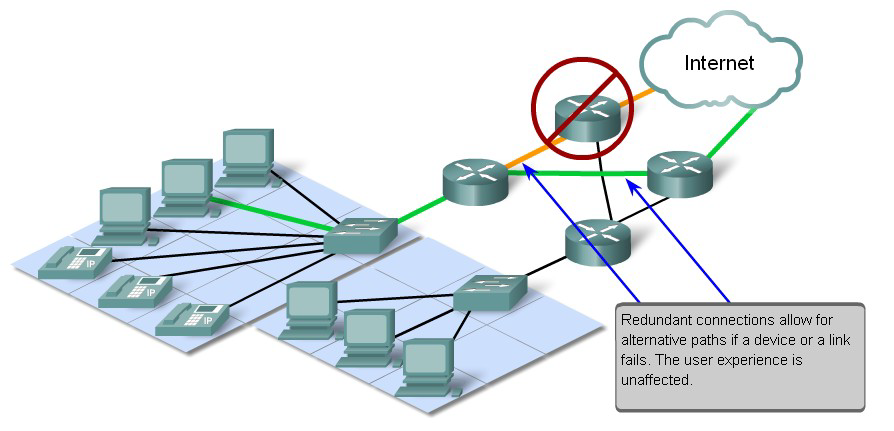
\includegraphics[scale=0.3]{DNet1_1.png} 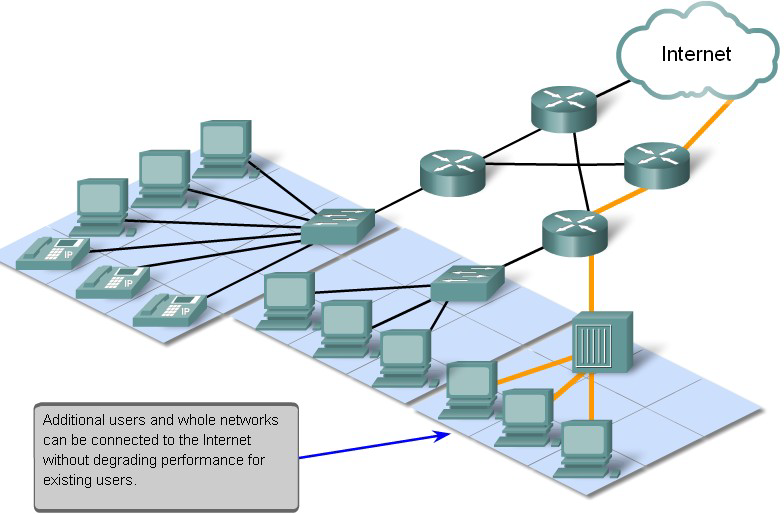
\includegraphics[scale=0.3]{DNet1_2.png}
\subsubsection{Leitungsvermittlung und Paketvermittlung}
\Bold{Leitungsvermittlung}  Bevor eine Kommunikation zwischen A und B bereitgestellt wird, wird ein Kanal zwischen den Telefonen hergestellt. WÀhrend der Anrufdauer werden alle Bits Ìber diesen Weg transportiert. Diese Art von Multiplexierung nennt man Time Division Multiplex (TDM). TDM-Netze zeichnen sich durch eine kleine und konstante Verzögerung des Signals und durch eine sehr hohe VerfÌgbarkeit aus.\\
\Bold{Paketvermittlung:} Pakete können unterschiedliche Wege nehmen, deshalb muss jedes Paket eine Adresse und andere Overheadinformationen, um ans Ziel zu gelangen. Jeder Netzknoten liest die Ziel-Adresse des Pakets und leitet es entsprechend weiter.\\
\Bold{Multiplexierung:} Sie erfolgt bei Paketvermittlung statistisch. Ganze Pakete verschiedenster Anwendungen und Herkunft werden nacheinander auf die Leitung multiplexiert. Ein Vorteil ist, dass wenn ein A keine Bandbreite belegt, mehr BB fÃŒr B zur VerfÃŒgung steht.
\subsubsection*{Vor- und Nachteile Tabelle}
\begin{tabular}{|l|l|l|}
 \hline
 &Vorteile&Nachteile\\\hline
 Leitungs-&$\bullet$ kleine Zeitverzögerung&$\bullet$ schlechte Auswertung der BB\\
 Vermittlung&$\bullet$ konst. Zeitverzögerung&$\bullet$ (maximale Anz. Teilnehmer)\\
 (verbindungs-&$\bullet$ hohe QualitÀt&$\bullet$ Kosten\\
 orientiert)&$\bullet$ Sicherheit&$\bullet$ limitierte BB (Bandbreite)\\\hline
 Paket-&$\bullet$ statistisch Multiplexen&$\bullet$ mehr Overhead\\
 Vermittlung&$\Ra$ bessere AusnÌtzung des Kanals&$\bullet$ Verzögerung ist ein Problem\\
 (verbindungs-&$\bullet$ gÃŒnstiger&$\Ra$ keine Garantien\\
 los)&&$\Ra$ keine Quality of Service, QoS\\
 &&$\bullet$ fÃŒr Sicherheit nun extra gesorgt werden\\\hline
\end{tabular}
\subsubsection{Skalierbare Netzwerkarchitektur des Internets}
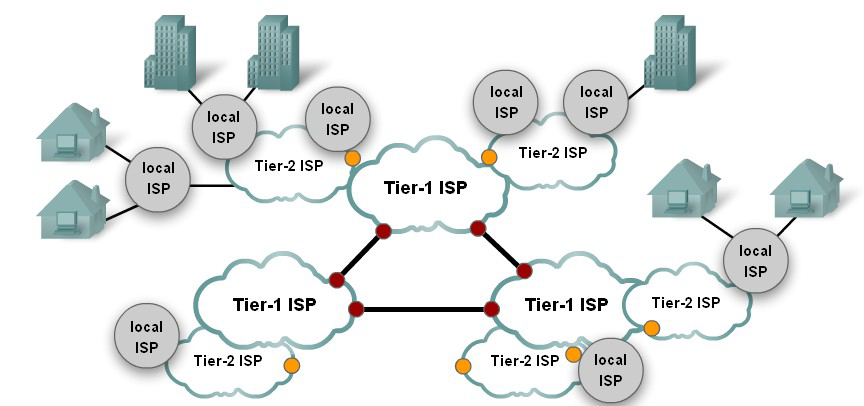
\includegraphics[scale=0.5]{DNet1_Tiers.png}\\
\Bold{Tier-1 ISP:} sind Internet Service Provider (ISP) die durch Leitungen mit einem sehr hohen Datendurchsatz miteinander verbunden sind.\\
\Bold{Tier-2 ISP:} Grosse ISP's schliessen sich an einem Tier-1 ISP an und sorgen dafÌr, dass der Verkehr innerhalb ihres Bereichs richtig lÀuft.\\
\Bold{Tier-3 ISP:} schliessen Endkunden an und zahlen Tier 2 ISP's fÃŒr den Zugang zum Internet.
\subsubsection{Was bei der Planung des Internets nicht berÃŒcksichtigt wurde}
\Bold{Quality of Service} (QoS)\\
Es geht soviel Verkehr durch das Netz, wie gerade KapazitÀten vorhanden sind. $\Ra$ Es werden keine KapazitÀten fÌr bestimmte Anwendungen reserviert. (keine QoS)\\
Verschiedene Dienste haben verschiedene Anforderungen an QoS:
\begin{itemize}
 \item Web
 \begin{description}
  \item[Durchsatz] hoch (Hoher Durchsatz in Downstream-Richtung)
  \item[Verzögerung] niedrig (keine Echtzeit Anforderungen)
  \item[Jitter] niedrig
  \item[Paketverluste] hoch (eine Datei muss fehlerlos ÃŒbertragen werden)
 \end{description}
 \item E-Mail
 \begin{description}
  \item[Durchsatz] \dots
  \item[Verzögerung] \dots
  \item[Jitter] \dots
  \item[Paketverluste] \dots
 \end{description}
 \item Voice over IP
  \begin{description}
  \item[Durchsatz] gering
  \item[Verzögerung] sehr empfindlich (Echtzeitanforderungen)
  \item[Jitter] sehr empfindlich
  \item[Paketverluste] gering
 \end{description}
\end{itemize}
\Bold{Sicherheit}\\
Bei der Definition der wichtigsten Internet Protokolle (IP, TCP, HTTP, SMTP, POP, FTP) wurde nicht an Sicherheit gedacht. SpÀter musste mÌhsam und mit viel Aufwand Sicherheit nachgebessert werden (Firewalls, SSL/TLS, IPsec).
\section{Schichtenmodelle für die Kommunikation über das Internet}
\subsection{Die Plattform für die Kommunikation}
Damit beim Multiplexieren nicht zu grosse Daten auf einmal verarbeitet werden müssen und so die Leitung blockiert, werden diese in Pakete von maximaler Länge unterteilt. Die Pakete brauchen Informationen um an das richtige Ziel zu gelangen, denn jedes Paket kann seinen eigenen Weg wählen.\\
\Bold{Netzkomponenten:} Endgeräte (Rechner, Printer, Telefone, Kameras, Sensoren) oder Netzwerkelemente ("Intermediary Devices" wie Router, Switch, Hub, Kommunikationsserver, Sicherheitsanwendungen)\\
Bei einer Kommunikation über das Internet können verschiedene Übertragungsmedien zum Zuge kommen: verdrillte Kupferdrähte, Glasfasern, Luft, Koaxialkabel
\subsection{LANs, WANs und Internetworks}
LAN: Local Area Network oder Limited Area Network\\
WAN: Wide Area Network\\
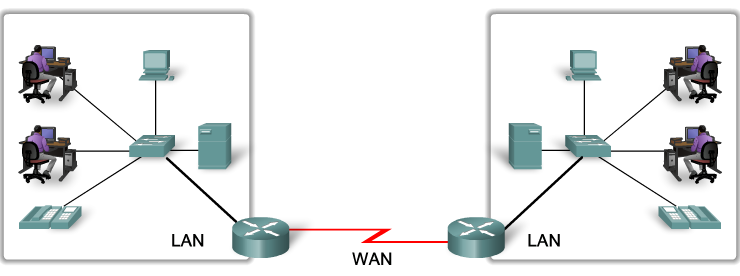
\includegraphics[scale=0.4]{DNet1_LAN_WAN.png}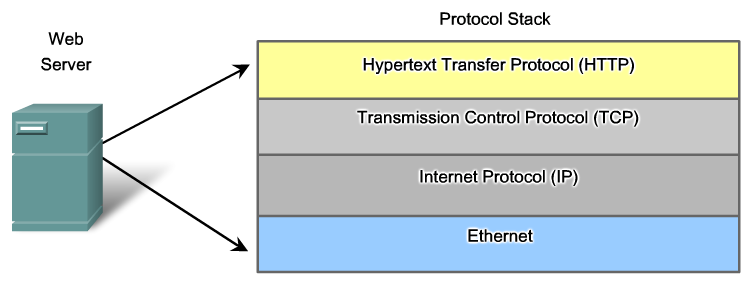
\includegraphics[scale=0.4]{DNet1_Protokollstack.png}
\subsection{Protokolle}
Ein Protokoll ist eine Regelsammlung, wie zwei Gegenüber miteinander kommunizieren sollen.
\subsection{Schichtenmodelle}
\subsubsection{Vorteile}
\begin{itemize}
 \item Man versucht komplexe Systeme mittels Schichten übersichtlicher und verständlicher darzustellen.
 \item Schichtenmodelle helfen, dass Produkte verschiedener Hersteller, zusammenarbeiten können.
 \item Schichtenmodelle helfen, dass für gewisse Funktionen neue Technologien eingesetzt werden können und das restliche System unverändert weiter läuft.
\end{itemize}
\subsubsection{Protokoll- und Referenzmodell}
\begin{description}
\item[Praxis] TCP/IP-Protokollstack
\item[Ausgangspunkt] Die Protokolle. Aus den Protokollen ergeben sich die Aufgaben, die eine Schicht abarbeitet (eher "bottom up").
\item[Theorie] OSI-Modell (Open System Interconnection). Damit erklärt man, welche abstrahierten Vorgänge in einer Schicht abgehandelt werden sollen. Dazu werden dann Protokolle entwickelt, die diese Aufgaben erfüllen (Top Down)
\end{description}


\end{document}
